\section{Diagrammi di sequenza}
Di seguito sono riportati i diagrammi di sequenza per quanto riguarda le operazioni principali del sistema.\\
Altri programmi di sequenza sono disponibili nel documento Definizione di Prodotto, sezione 7 (\textit{\DefinizioneDiProdotto}).

	\subsection{Verifica dell'esistenza dello username}
		\begin{center}
			\begin{figure}[htbp]
				\centering
				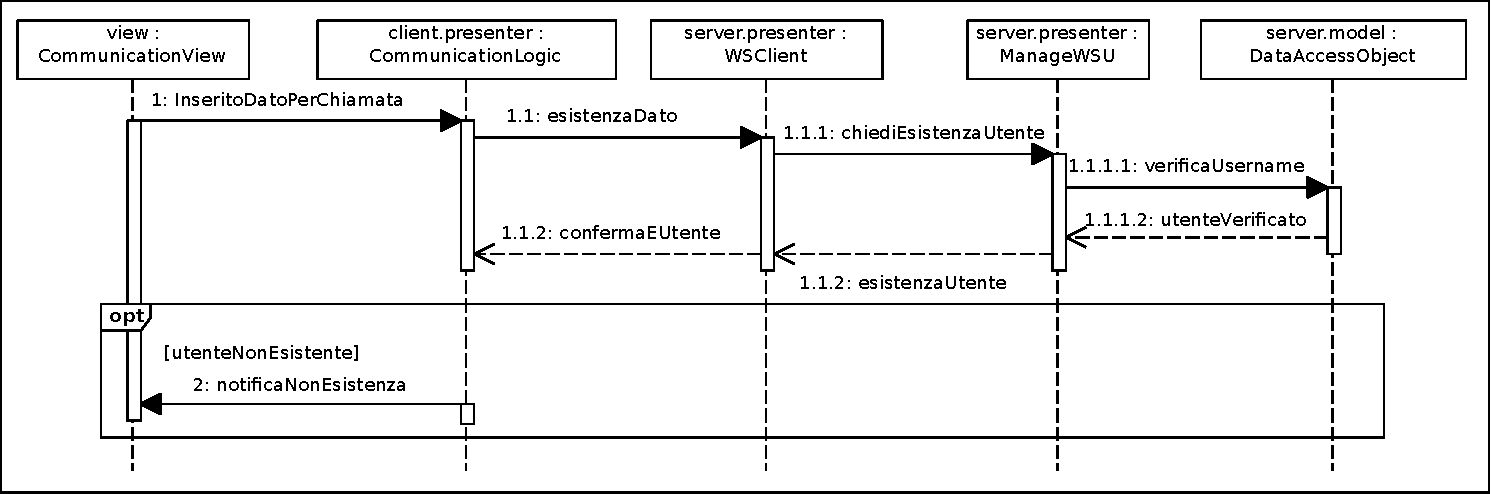
\includegraphics[scale=0.7]{\docsImg /immagini.diagrammi/esistenzaUsername.pdf}
			\caption{DS 1 - La procedura di verifica dell'esistenza di un utente di cui si conosce un dato.}	
			\end{figure}
		\end{center}	
	\noindent \textbf{Precondizione: }l'utente vuole chiamare un altro utente inserendo un dato, username o indirizzo IP\g , che identifica univocamente l'utente da chiamare.\\
	\textbf{Descrizione: }il diagramma mostra la procedura con la quale il sistema verifica se il dato inserito dall'utente è associabile univocamente ad un utente presente nel database\g.\\
	La classe \texttt{CommunicationView} genera l'evento associato all'inserimento di un dato che viene ricevuto dalla classe \texttt{CommunicationLogic}, la quale:
	\begin{enumerate}
	\item estrapola il dato inserito dall'utente sotto forma di testo;
	\item invia il dato, tramite WebSocket\g , alla classe \texttt{WSUser} che risiede all'interno del server\g ;
	\item la classe \texttt{WSUser} invia il dato alla classe \texttt{DataAccessObject}, che gestisce il DBMS\g , la quale tramite una ricerca all'interno della base di dati, ritorna un valore che indica se il dato passato è associabile ad un utente univoco oppure no;
	\item il risultato, identificabile con un booleano\g, viene restituito alla classe\\ \texttt{CommunicationLogic}, la quale in questo modo ha scoperto se esiste un utente al quale corrisponde il dato inserito dall'utente. Se la risposta è negativa, la classe \texttt{CommunicationLogic} notifica la non esistenza dell'utente alla classe \texttt{CommunicationView}.
	\end{enumerate}
	\textbf{Postcondizione: }l'utente sa se l'utente che vuole chiamare esiste oppure no. Il sistema è pronto a creare il gestore della connessione.